\documentclass[addpoints,12pt,answers]{exam}
\usepackage{babel}
\usepackage[top=3cm,bottom=3cm,left=2.5cm,right=2.5cm]{geometry}
\usepackage[utf8]{inputenc}
\usepackage[T1]{fontenc}
\usepackage{booktabs}
\usepackage{graphicx}
\usepackage{csquotes}
\usepackage{paralist}
\usepackage{wasysym}
\usepackage[math]{iwona}
\usepackage{setspace}
\usepackage{enumitem}


\pointpoints{Point}{Points}
\bonuspointpoints{Bonuspunkt}{Bonuspunkte}
\renewcommand{\solutiontitle}{\noindent\textbf{Solution:}\enspace}

\chqword{Frage}   
\chpgword{Seite} 
\chpword{Punkte}   
\chbpword{Bonus Points} 
\chsword{Erreicht}   
\chtword{Gesamt}

\checkboxchar{\Square}
\checkedchar{\CheckedBox}

\pagestyle{headandfoot}
%\runningheadrule
%\firstpageheader{ECO208}{Test 3}{28th Feb, 2022}
%\runningheader{ECO208}{Test 3}{28th Feb, 2022}
%\firstpagefooter{ECO208}{Test 3}{\thepage\,/\,\numpages}
%\runningfooter{ECO208}{Test 3}{\thepage\,/\,\numpages}
\doublespacing

\begin{document}
	\vspace*{3em}
	
	\makebox[\textwidth]{ECO 209  Assignment 1 }
	\makebox[\textwidth]{Name:\enspace\hrulefill}
	
	\vspace*{3em}
	
	\begin{questions}
		
		
		\question  [20]  Suppose a country’s economy can be fully described by the following activities:
		
		- A gold mining company pays its workers \$2800 to mine and process 100 kg of gold. The company sells 80 kg to a decoration manufacturer and forges 10 gold bars, which are sold directly to consumers for \$5000.
		
		- A decoration manufacturer buys 80kg of gold at \$100 per kg and pays its workforce \$21,000 to produce 7 gold decorations. Out of these, 4 are sold to end consumers, 1 to a government-run museum, and 2 are exported for \$12,000 each.

		
		\begin{enumerate}[label=(\alph*)]
			\item (\textbf{12 pts}) Calculate the GDP in the economy using all three methods. Please show your work in detail.
			\item (\textbf{3 pts}) Suppose that in the following year, the amounts of gold mined and gold decorations produced remain the same, wages paid by both firms remain the same, but the price of gold is now \$110 per kg, and the price of a decoration is \$15,000.
			
			What is the growth rate of real GDP between the first year and the next? Explain your answer.
			\item (\textbf{5 pts}) Using the GDP deflator method, calculate the percentage change in the general price level across the two years. Show your work.
		\end{enumerate}
		
		\clearpage
		\begin{solution}
			\begin{parts}
				\item 
				Using the income approach, we need to sum all the labour income and capital income. The labour income consists of \$2,800 from the gold mining company and \$21,000 from the decoration manufacturer. The business owner's earnings are calculated as revenue minus costs. 
				
				For the gold mining company, the owner earns \$100 (the price per unit) multiplied by 80 (units produced), which is \$8,000 in revenue. Also, the owner earn \$5000 from selling gold bar directly to consumer. Subtracting the labour cost of \$2,800, the owner's earnings are \$10,200. 
				
				For the decoration manufacturer, the owner earns 7  multiplied by \$12,000 (the price per unit) (units produced) minus the costs (\$21,000  for labour and \$8,000 for materials), resulting in earnings of \$55,000. 
				
				Summing all the labour and capital income:
				
				\[
				GDP = \$2,800 + \$10,200 + \$21,000 + \$55,000 = \$89,000
				\]
				
				Using the expenditure approach, we need to sum all the final goods consumption, which is:
				
				\[
				GDP = C + G + NX = \$5000 + 4 \times \$12,000 + 1 \times \$12,000 + 2 \times \$12,000 = \$89,000
				\]
				
				Using the value-added approach, we first calculate the value added for each firm. For the gold mining company, it doesn't incur any intermediate costs, so its value added is the revenue, which is \$13,000. For the decoration manufacturer, its value added is \$84,000 (revenue) minus \$8,000, resulting in \$76,000.
				
				\[
				GDP = \$13,000 + \$76,000 = \$89,000
				\]
				\item 
				Real GDP remains unchanged as production quantities remain constant. The only variable that changes is the price. Therefore, the growth rate is zero. 
				\item 
				First, use any method to find the nominal GDP in the next year $= \$5000 + \$15000*7 = \$110,000$
				
				Now, find the GDP Deflator = NGDP/RGDP = 110,000/89,000= 1.24
				
				Percentage change in prices = (1.24-1)*100\% = 24\%
			\end{parts}
		\end{solution}
		\clearpage
	

		\clearpage
		\question  [10]  Suppose $x$, $y$, and $z$ grow at constant rates given by $\bar{x}$, $\bar{y}$ and $\bar{z}$. What is the growth rate of $z$ in each of the following cases?
		\begin{enumerate}[label=(\alph*)]
			\item (\textbf{2 pts}) $z=xy$
			\item (\textbf{4 pts}) $z=x^{-0.4} \left(\frac{1}{y}\right)^{0.2}$
			\item (\textbf{4 pts}) $z= \frac{y^{0.3}}{x^{0.2}}$
		\end{enumerate}
		\clearpage
		\begin{solution}
			\begin{parts}
				\item $g_z = g_x+g_y$
				\item $g_z = g(x^{-0.4}) + g\left(\left(\frac{1}{y}\right)^{0.2}\right) = -0.4g_x + 0.2g(1/y) = -0.4g_x +0.2g(y^{-1}) = -0.4g_x -0.2g_y$
				\item $z=y^{0.3}x^{-0.2}$, $g_z = 0.3g_y -0.2g_x$
			\end{parts}
		\end{solution}
		
		\clearpage
		\question  [10] Suppose that country A is growing at 3\% per year, and country B is growing at 2\%. In the year 2000, the GDP per capita of country A is \$8,000, and the GDP per capita of country B is \$30,000.
		
		\begin{enumerate}[label=(\alph*)]
			\item (\textbf{5 pts}) How long would it take country A to catch up with country B in term of GDP per capita?
			\item (\textbf{5 pts}) With the help of foreign investment and technology diffusion, country A can grow at 5\% in the initial 20 years. How long would it take for country A to catch up with country B in this case? (Hint: If a country is growing at 2\% in the first 2 years and the growth rate falls to 1\%, we can calculate the GDP after 5 years as $Y_5 = Y_0(1.02)^2(1.01)^3$.)
		\end{enumerate}
		\clearpage
		\begin{solution}
			\begin{parts}
				\item To calculate that, we set the GDP in year t for country A and country B to be equal.
				\[Y^A_t =Y^B_t\]
				We can apply the constant growth rate formula
				\[Y^A_0 (1+g_A)^t = Y^B_0 (1+g_B)^t \]
				\[8000 (1.03)^t = 30000 (1.02)^t  \to \left(\frac{1.03}{1.02}\right)^t = 3.75\]
				\[\ln\left(\frac{1.03}{1.02}\right)^t = ln\left(3.75\right) \to t\ln\left(\frac{1.03}{1.02}\right) = ln\left(3.75\right)\]
				\[t= 135.48\]
				\item The procedure is similar except that for the first 20 years, the growth rate for country A is at 5\%
				\[8000 (1.05)^{20}(1.03)^{t-20} = 30000 (1.02)^t\]
				\[\frac{(1.03)^{t}}{(1.03)^{20}(1.02)^t} = \frac{30000}{8000 (1.05)^{20}} \to \left(\frac{1.03}{1.02}\right)^t = \frac{30000}{8000 (1.05)^{20}} (1.03)^{20}\]
				\[t \ln\left(\left(\frac{1.03}{1.02}\right)\right) = \ln\left(\frac{30000}{8000 (1.05)^{20}} (1.03)^{20}\right)\]
				\[t = 96.05\]
			\end{parts}
		\end{solution}
		
		\clearpage
		\question  [15] Do the following production functions exhibit increasing, constant, or decreasing returns to scale in both $K$ (capital) and $L$ (labour)? ($\bar{A}$ is a fixed positive number)
		\begin{enumerate}
			%\item \textbf{5 pts} $Y=K+L$
			\item (\textbf{5 pts}) $Y=\bar{A}K^{1/3}L^{1/2}$
			\item (\textbf{5 pts}) $Y=K^{1/3}L^{2/3} - \bar{A}$
			\item (\textbf{5 pts}) $Y= L+K^{0.5}L^{0.5}$
		\end{enumerate}
		
		\begin{solution}
			When the production function is not Codd-Douglas, we will check the return to scale by multiply the input by $\gamma$ 
			\begin{parts}
				%\item $\gamma K + \gamma L = \gamma (K+L) = \gamma Y$. Constant return to scale
				\item The sum of $\frac{1}{3} + \frac{1}{2} <1$. Decreasing return to scale
				\item Although the sum of $1/3+2/3 = 1$, we are subtracting it by a constant term $\bar{A}$. We cannot tell what kind of return to scale by checking the power. Sub it $K=\gamma K$ $L=\gamma L$
				\[F(\gamma K, \gamma L) - \gamma F(K,L) = \gamma K^{1/3}L^{2/3} - \bar{A} - \gamma \left(K^{1/3}L^{2/3} - \bar{A}\right)\]
				\[\gamma K^{1/3}L^{2/3} - \bar{A} - \gamma K^{1/3}L^{2/3} + \gamma \bar{A} = (\gamma-1) \bar{A}\]
				So, the function is increasing return to scale
				\item $\gamma L+(\gamma K)^{0.5} (\gamma L)^{0.5} = \gamma L+ \gamma( K)^{0.5} ( L)^{0.5} = \gamma \left(L+K^{0.5}L^{0.5}\right)$. Constant return to scale
			\end{parts}
		\end{solution}
		
		\clearpage
		\question  [25]	This question relates to the Solow growth model discussed in Chapter 5. Mont Plaisant, a closed economy with no government spending, operates under the following production function:
		\[
		Y_t = A K_t^{1/3} L_t^{2/3}
		\]		
		In this model, \(Y_t\) represents the output in period \(t\), \(K_t\) denotes the capital stock in period \(t\), and \(L_t\) stands for the labour employed in period \(t\). The accumulation of capital follows the standard equation:
		\[
		K_{t+1} = (1 - \delta) K_t + I_t
		\]		
		where \(\delta\) is the depreciation rate and \(I_t\) is the investment in period \(t\).
		
		Mont Plaisant's population saves a fixed proportion, \(\bar{s}\), of their output for investment each period. The population grows at a rate \(\bar{n}\), following the equation \(L_{t+1} = (1 + \bar{n}) L_t\). Lowercase letters represent per-person values of the variables.
		
		\begin{enumerate}[label=(\alph*)]
			\item Convert the capital accumulation equation from aggregate to per-person terms. The left-hand side should equal \(\Delta k_{t+1}\), while the right-hand side should include \(y_t\), \(k_t\), and the relevant parameters.
			
			\item Find the steady-state values of capital per capita (\(k^*\)) and output per capita (\(y^*\)).
			
			\item What happens to output per capita in the steady state when \(\bar{s}\) increases? Use your findings from part (b) to explain.
			
			\item After estimating the model, we have the following parameter values and exogenous variables: \(\delta = 0.05\), \(\bar{A} = 1\), \(\bar{s} = 0.20\), and \(\bar{n} = 0.02\). Additionally, the current capital per capita in period 1 is \(k_1 = 4\). Using this information, calculate \(\Delta k_2\), \(\Delta k_3\), \(\Delta k_4\) and $\Delta k_5$. What pattern do you observe in \(\Delta k_t\), and why does this pattern occur? Explain in 2-4 sentences.
			
			\item How should we expect the growth rate of output in Mont Plaisant from period 1 onward? Explain in 2-4 sentences.
			
			\item Draw a Solow diagram with \(k\) on the x-axis to illustrate the scenario described in part (d).
			%			
			%			\item Draw two separate time graphs (on a ratio scale) for $Y$ and $y$, one for Mont Plaisant and the other for Mont-Tremblant.
			\end{enumerate}

		
		
		
		\newpage
		\textbf{Solution:}
		\begin{enumerate}[label=(\alph*)]
			\item Plug in ($I_t = s Y_t$)
			\[K_{t+1}- K_t = \Delta K_{t+1}=  sY_t -\delta K_t\]
			Divide both side by $K_t$,
			\[\frac{\Delta K_{t+1}}{K_t} = g_K  = s\frac{Y_t }{K_t}-\delta = s\frac{Y_t/L_t }{K_t/L_t}-\delta = s\frac{y_t }{k_t}-\delta\]
			Now, recall that $k_t = \frac{K_t}{L_t}$ and apply the growth rate approximate formula:
			\[g_k = g_K - g_L\]
			
			Next, plug in the $g_K$ above and the fact that $g_L = \bar{n}$
			\[g_k= \frac{\Delta k_{t+1}}{k_t} = s\frac{y_t }{k_t}-\delta - \bar{n}\]
			Multiply both sides by $k_t$
			\[\Delta k_{t+1} = sy_t- (\delta + \bar{n})k_t\]
			\item 
			In steady state, $\Delta k_{t+1} = 0$
			\[0 = sy^*- (\delta + \bar{n})k^*\]
			\[(\delta + \bar{n})k^* = sy^* \]
			\[\frac{k^*}{y^*} = \frac{s}{\delta + \bar{n}} \]
			
			Rearrange the equation to $k^* = \frac{s}{\delta + \bar{n}} y^*$ and plug it into the output function ($y_t = Ak^{1/3}_t$):
			\[y^* = A \left(\frac{s}{\delta + \bar{n}} y^*\right)^{1/3}\]
			\[y^{* 2/3} = A \left(\frac{s}{\delta + \bar{n}} \right)^{1/3}\]
			\[y^{*} = A^{3/2} \left(\frac{s}{\delta + \bar{n}} \right)^{1/2}\]
			
			The steady-state $k^*$ is then
			\[k^* =  A^{3/2}  \left(\frac{s}{\delta + \bar{n}} \right)^{3/2}\]
			
			\item We can use the formula we derived earlier to calculate the change in capital per person. 
			
			\[\Delta k_{t+1} = sy_t- (\delta + \bar{n})k_t\]
			
			$\Delta k_2 = 0.037$, $\Delta k_3 = 0.036$, $\Delta k_4 = 0.034$, and $\Delta k_5 = 0.031$.
			
			We observe that the change in capital is positive, meaning capital increases each period, but at a decreasing rate. This occurs because the economy is currently below its steady state. But,			as the economy approaches the steady state, the growth rate gradually declines.
			
			\item Since the economy is currently below its steady state, the economy will experience positive growth in output. It is because  there will be positive net investment (i.e., \(sy_t > (\delta + \bar{n}) k_t\)), leading to capital growth in addition to population growth. The growth rate would slow down as the economy get closer to the steady state.
			
			\item
			\begin{figure}[htbp!]
				\centering
				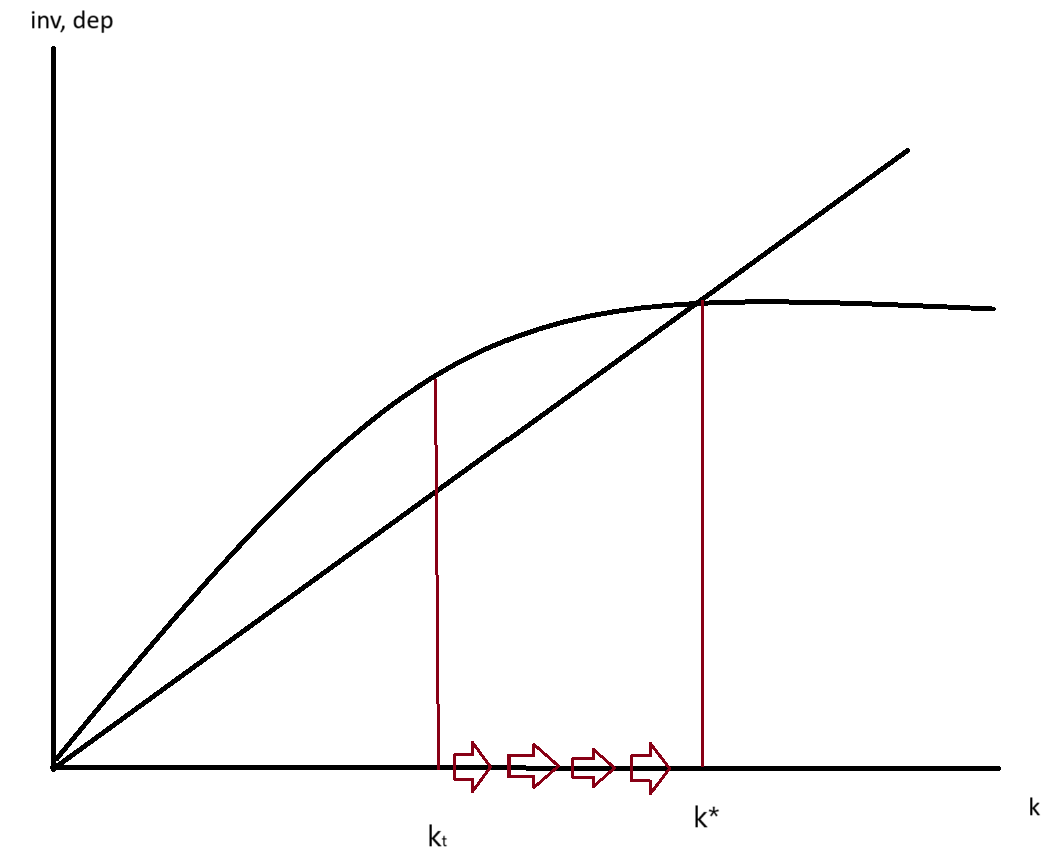
\includegraphics[width=0.7\linewidth]{figure/fig9}
			\end{figure}
			

		\end{enumerate}
		
	%	\clearpage 
%		\question [20] Data Question: 
%		\begin{parts}
%			\item \textbf{4 pts} Download two data series \textit{(i)} ``Real GDP at Constant National Prices for Japan, Annual [RGDPNAJPA666NRUG], retrieved from FRED, Federal Reserve Bank of St. Louis'' and \textit{(ii)} ``Population, Total for Japan, Annual [POPTOTJPA647NWDB]'' data series from https://fred.stlouisfed.org from 1960 to 2016. Both data should be on the same data sheet. (Hints: (1) You can search the code inside the square bracket on the FRED website for the data (2) Use ``Edit Graph'' --> ``Add Line'' to add another data series on the same sheet)
%			\item [6] In a new column, calculate the Real GDP per capita. Then, in another column, log-transform the calculated Real GDP per capita. Submit this part as a screenshot of the spreadsheet. The original data should not be alternated! (Note that the Real GDP data is in millions of 2017 U.S. dollars. Convert it to dollars when calculating the Real GDP per capita.)
%			\item [6] Plot two time-series graph (i.e., the variables of interest on the Y-axis and time on the X-axis). The first figure shows Real GDP per capita calculated in part b). The second figure shows the log-transformed Real GDP per capita. Provide the y-axis title, x-axis title, and chart title. Then, adjust the x-axis to display only the year, excluding the month and day.
%			\item \textbf{4 pts} Does the real GDP per capita exhibit exponential growth? What does the log-transformed Real GDP per capita reveal about the growth in Japan?
%			\item [10] Conduct a brief Research on Japan's Lost Decade. What factors contributed to Japan's long-term recession? Provide a summary in 5-8 sentences, focusing either on a specific cause or giving an overview of the recession.
%		\end{parts}
		
%		\newpage 
%		\centering{This page intentionally left blank.}
%		\ % The empty page
%		

		
%		 \centering{-- The End -- }
		
		
		
		%		\begin{solution}
			%			
			%		\end{solution}	
%		\clearpage 
%		
%		\question Was wäre, wenn es keine Luft gäbe?
%		\begin{parts} 
%			\item\textbf{5 pts} Was würde mit Luftballons geschehen? 
%			\bonuspart[6] Wie könnten Fluggesellschaften damit umgehen?
%		\end{parts}
%		
%		\question [100] Wird es morgen schneien?
%		\begin{checkboxes}
%			\CorrectChoice Ja
%			\choice Nein
%			\choice Vielleicht
%		\end{checkboxes}
%		
%		\question Ein Name der folgenden Reihe passt nicht zu den anderen. Welcher?
%		\begin{oneparchoices}
%			\choice Donald
%			\choice Dagobert
%			\choice Daisy
%			\choice Micky
%			\CorrectChoice Balu
%		\end{oneparchoices}
		
	\end{questions}
	
%	\begin{center}
%		\combinedgradetable[h][questions]
%	\end{center}
	
\end{document}